\chapter{Herramientas y técnicas}
Para mantener el presente documento, así como para detectar nuevos riesgos y redactar sus respectivos planes de gestión, se utilizarán las siguientes técnicas:
	\begin{itemize}
		\item Puesta en común de nuevos riesgos siempre que cualquiera de los integrantes del proyecto crea detectar uno.
		\item Puesta en común del resultado de aplicar los planes de gestión. Dará lugar a propuestas de mejora de los planes de gestión de riesgos ya detectados.\\
	\end{itemize}
	
El encargado de mantener el documento de gestión de riesgos deberá:
	\begin{itemize}
		\item Evaluar la probabilidad de aparición e importancia de cada uno de los nuevos riesgos.	Para cada uno de ellos, si considera que tienen una probabilidad o importancia relevantes, se encargará de preparar un plan de gestión de riesgos para el nuevo riesgo. Por otra parte, si un riesgo es similar a otro ya contemplado, se podrá extender un plan de gestión de riesgos existente para que contemple el nuevo caso.
		\item Revisar los planes de gestión de los riesgos ya tratados en base a las observaciones hechas por quienes los aplicaron.\\
	\end{itemize}
	
Todo el equipo deberá:
	\begin{itemize}
		\item Estar al tanto de la existencia de este documento, así como de los riesgos que se contemplan en él.
		\item Tener una idea general del plan de gestión de cada riesgo.
		\item Consultar el plan de gestión de un riesgo contemplado en este documento tan pronto como se presente.\\
\\
\\
\\
\\
	\end{itemize}
		
Se seguirá la clasificación de riesgos propuesta por Boehm, que aparece en la siguiente figura:\\
\begin{tabbing}
---- \= ------ \= ----- \kill
\>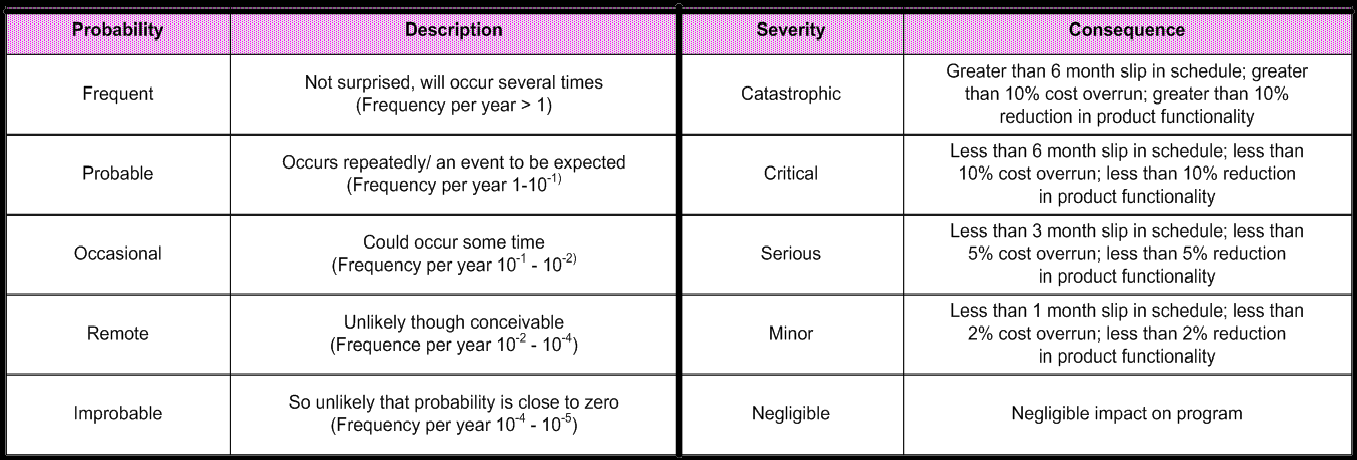
\includegraphics[width=0.96\textwidth]{7.PlanDeGestionDeRiesgos/Imagenes/ClasificacionRiesgosBoehm}
\end{tabbing}